\section{Financial network topology}
\label{sec:networks}

Clustering summarises hierarchical organisation, but it does not identify graph-theoretic hubs, bridges or local cycles. Financial networks provide these complementary views by retaining selected high-correlation, short-distance edges under structural constraints. We therefore move from dendrograms to filtered financial networks to examine how dependency topology changes after RMT filtering.

\subsection{MST backbone}

The MST is the sparsest connected representation of the dependency geometry. With $N=58$, it contains 57 edges. Figure~\ref{fig:mst_refined} compares the MST built from the original matrix with the MST built from the group-mode matrix. This comparison illustrates how the MST backbone changes after the leading market component is removed.

\begin{center}
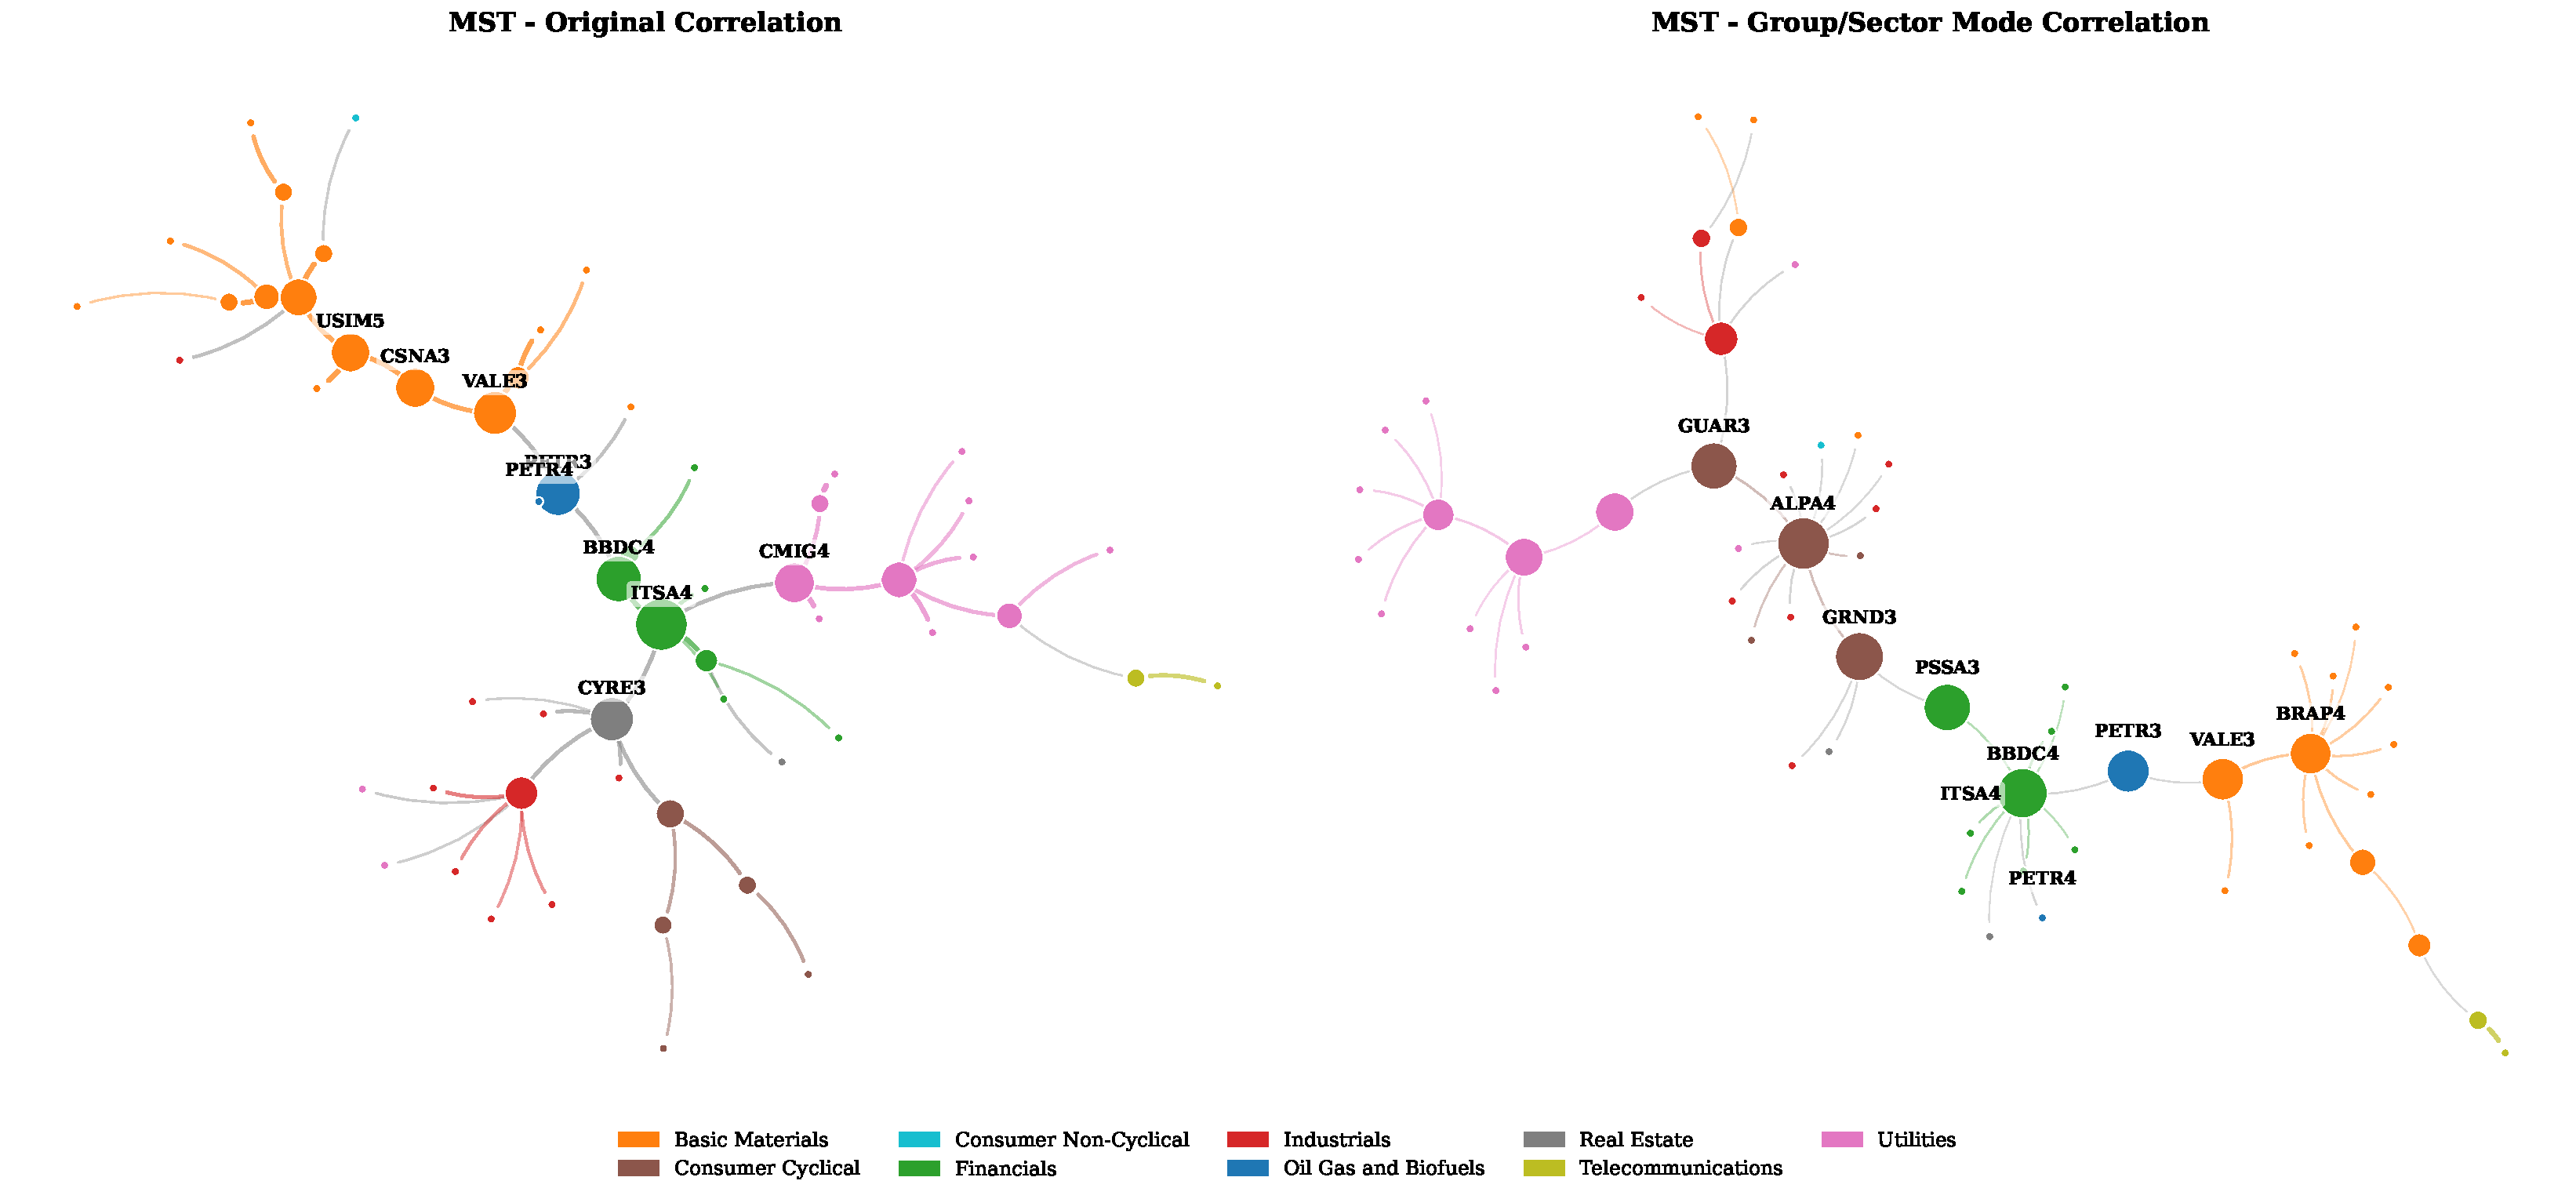
\includegraphics[
  width=\linewidth,
  height=0.58\textheight,
  keepaspectratio
]{images/figure_11b_mst_refined_comparison.pdf}
\captionof{figure}{Refined MST comparison for original and group-mode correlation matrices. The original MST emphasizes strong market-mode dependencies, while the group-mode MST highlights weaker localized dependency channels.}
\label{fig:mst_refined}
\end{center}

The original MST has mean edge correlation 0.5796, while the group-mode MST has mean edge correlation 0.1388. This decline is expected because the group-mode network is constructed after excluding the dominant common component. The same-sector edge ratio also changes, from 0.7193 in the original MST to 0.6316 in the group-mode MST. The group-mode MST should therefore not be interpreted simply as a weaker version of the original tree. It represents a different dependency backbone constructed after removing the leading common component.

\subsection{PMFG topology}

The PMFG is less sparse than the MST because it preserves planarity while retaining $3N-6=168$ edges. It can therefore retain cycles, triangles and 4-cliques, which are absent from the MST. Figure~\ref{fig:pmfg_refined} compares original and group-mode PMFGs. This is the main network visualization in the paper because the PMFG retains enough structure to study local connectivity patterns, clustering and hub reorganization.

The original PMFG has mean edge correlation 0.5177. The group-mode PMFG has mean edge correlation 0.1109. Despite this lower average edge strength, the group-mode PMFG has higher average clustering, 0.6653, than the original PMFG, 0.5273. This is an important result: removing the market mode lowers the absolute level of edge correlations, but the resulting PMFG is associated with stronger local clustering.

\begin{center}
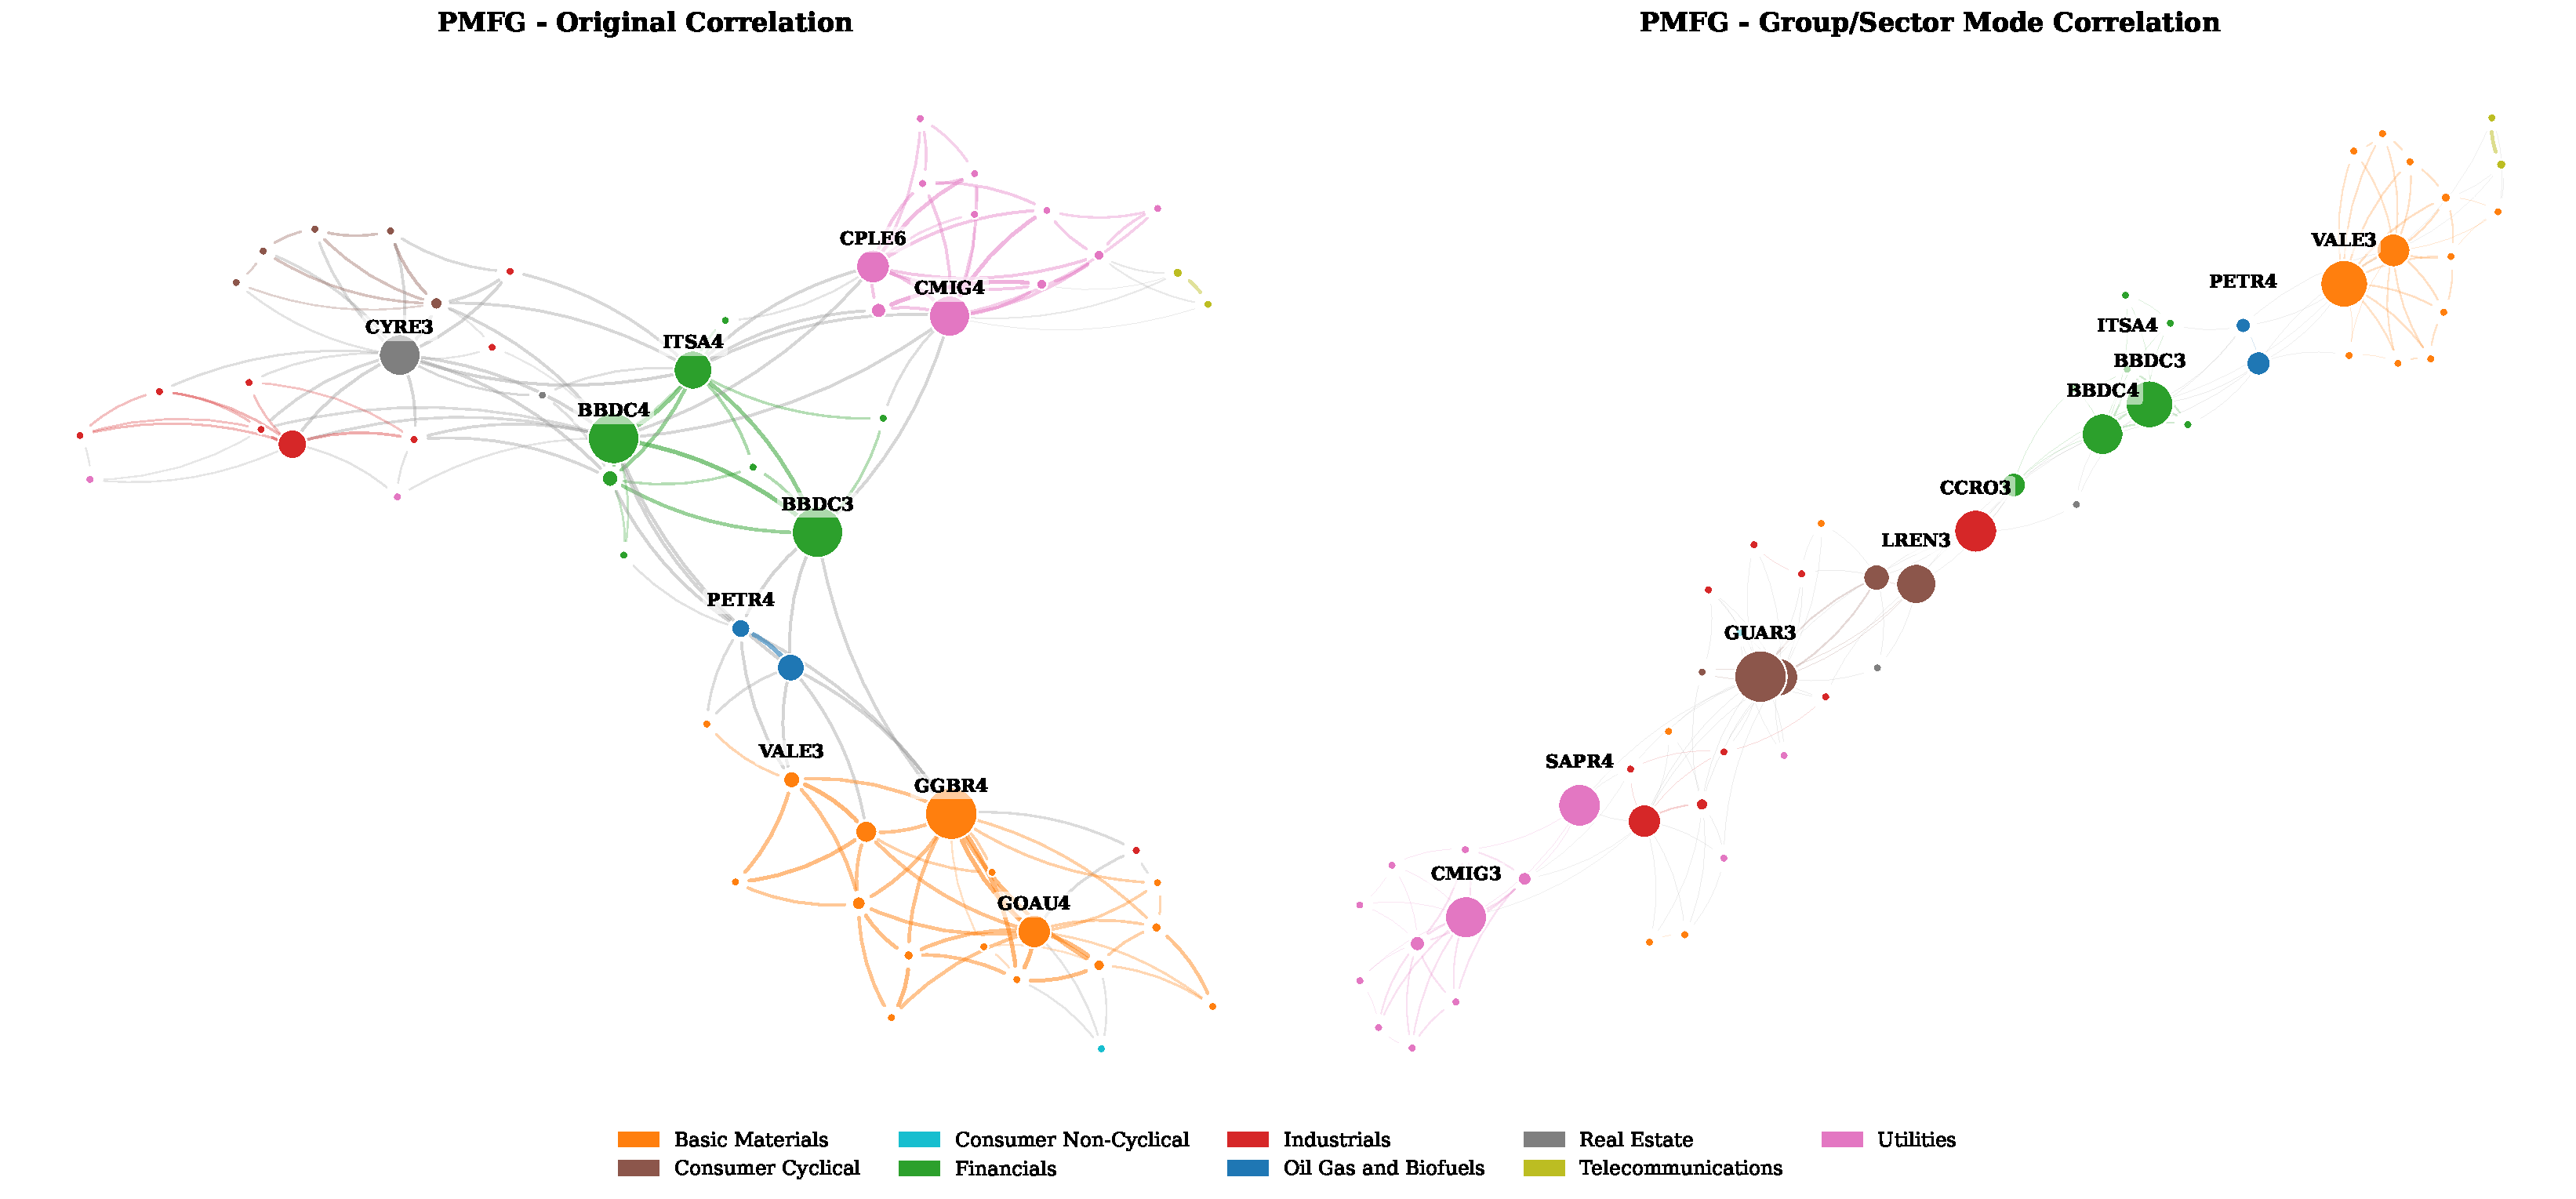
\includegraphics[
  width=\linewidth,
  height=0.58\textheight,
  keepaspectratio
]{images/figure_12b_pmfg_refined_comparison.pdf}
\captionof{figure}{Refined PMFG comparison for original and group-mode correlation matrices. The group-mode PMFG reduces market-wide dominance and highlights more localized dependency channels.}
\label{fig:pmfg_refined}
\end{center}


\subsection{Original vs Group/Sector Mode networks}

Table~\ref{tab:network_summary} summarizes the main MST and PMFG statistics. Across both graph families, original networks display stronger average edge correlations, while group-mode networks display weaker edge correlations but retain nontrivial sectoral and topological structure. Original networks have stronger average edge correlations, as expected, because they are constructed from matrices that include the leading market component. Group-mode networks have weaker edges but retain patterns consistent with sectoral and subsectoral organization.

\begin{center}
\captionof{table}{Selected MST and PMFG topology statistics.}
\label{tab:network_summary}
\resizebox{\linewidth}{!}{%
\begin{tabular}{llrrrrrrr}
\toprule
Network & Matrix & Edges & Mean edge corr. & Same-sector ratio & Clustering & Top degree & Top betweenness & 4-cliques \\
\midrule
MST & Original & 57 & 0.5796 & 0.7193 & 0.0000 & RAPT4 & ITSA4 & 0 \\
MST & Group mode & 57 & 0.1388 & 0.6316 & 0.0000 & ALPA4 & ALPA4 & 0 \\
PMFG & Original & 168 & 0.5177 & 0.6012 & 0.5273 & BBDC4 & GGBR4 & 55 \\
PMFG & Group mode & 168 & 0.1109 & 0.5417 & 0.6653 & GUAR3 & GUAR3 & 55 \\
\bottomrule
\end{tabular}}
\end{center}

\subsection{Network topology metrics}

Figure~\ref{fig:network_topology} expands the comparison beyond average edge correlation. It summarizes mean edge correlation, same-sector ratio, same-subsector ratio and average clustering across network and matrix types. This figure illustrates that topology should not be reduced to a single edge-weight statistic.

The topology comparison supports a mesoscopic interpretation. Group-mode networks have lower mean edge correlations, while the PMFG clustering coefficient increases. Same-sector and same-subsector ratios remain substantial after market-mode removal. This pattern is consistent with localized dependency structure, although a formal comparison with graph null models would be required to quantify how unlikely the topology is under randomized alternatives. MST clustering is zero by construction because trees do not contain triangles; the PMFG clustering coefficient is therefore the relevant statistic for local triangular organization.

\begin{center}
\captionof{table}{PMFG clique and planarity diagnostics.}
\label{tab:pmfg_cliques}
\begin{tabular}{lrrrrl}
\toprule
Matrix & Nodes & Edges & Triangles & 4-cliques & Planar \\
\midrule
Original & 58 & 168 & 166 & 55 & Yes \\
Filtered & 58 & 168 & 166 & 55 & Yes \\
Group Mode & 58 & 168 & 166 & 55 & Yes \\
\bottomrule
\end{tabular}
\end{center}

The clique counts are construction diagnostics. For a PMFG with 58 nodes, 168 edges are expected. The presence of triangles and 4-cliques shows that the PMFG retains local topological structures that are absent from the MST. These structures can be transformed into network predictors for the forecasting experiment, although their economic interpretation depends on the underlying edge weights and sector composition.


\begin{center}
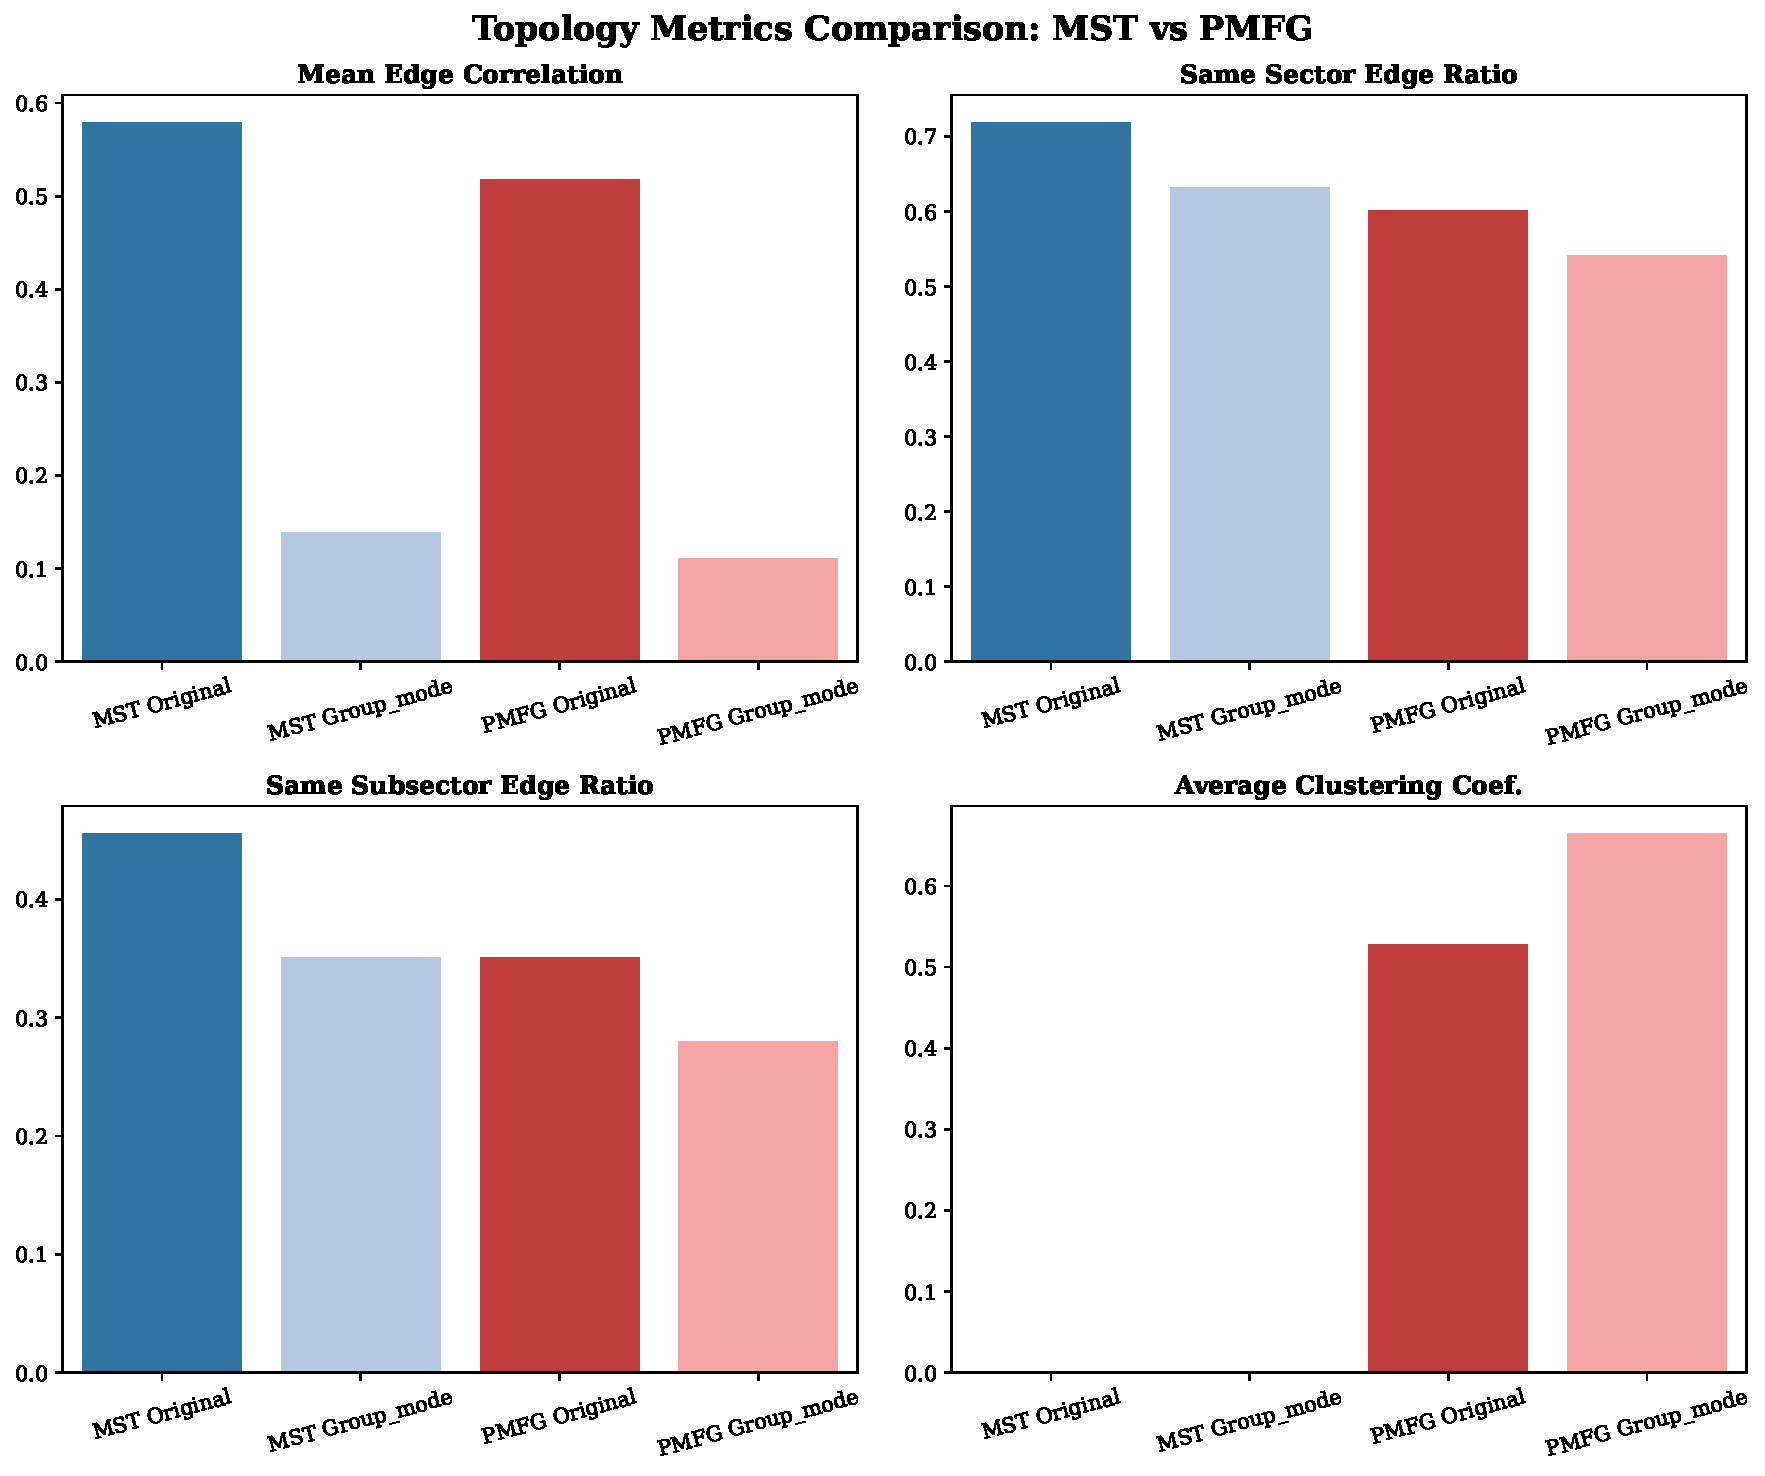
\includegraphics[
  width=\linewidth,
  height=0.58\textheight,
  keepaspectratio
]{images/figure_13_network_topology_comparison.pdf}
\captionof{figure}{Network topology comparison across original, filtered and group-mode MST/PMFG representations.}
\label{fig:network_topology}
\end{center}

\subsection{Hub reorganization after RMT filtering}

Hub rankings summarize which assets occupy central positions in the constructed networks. Figure~\ref{fig:hub_rank} compares hub rankings before and after filtering. In the original PMFG, GGBR4 is the top betweenness node and BBDC4 is the top degree node. In the group-mode PMFG, GUAR3 becomes the leading node by both degree and betweenness.

This change in hub ranking is informative for interpretation. Original hubs can reflect market-wide correlation strength and broad exposure to the common component. Group-mode hubs are interpreted as localized bridges in the network obtained after removing the leading common component. The appearance of assets such as GUAR3, BBDC3, VALE3, CCRO3, SAPR4 and CMIG3 in group-mode rankings suggests that centrality should be interpreted conditionally on the matrix used to construct the network. Because hub identities can be sensitive to small changes in edge ranking, these rankings are interpreted as descriptive summaries rather than stable structural labels.

\begin{center}
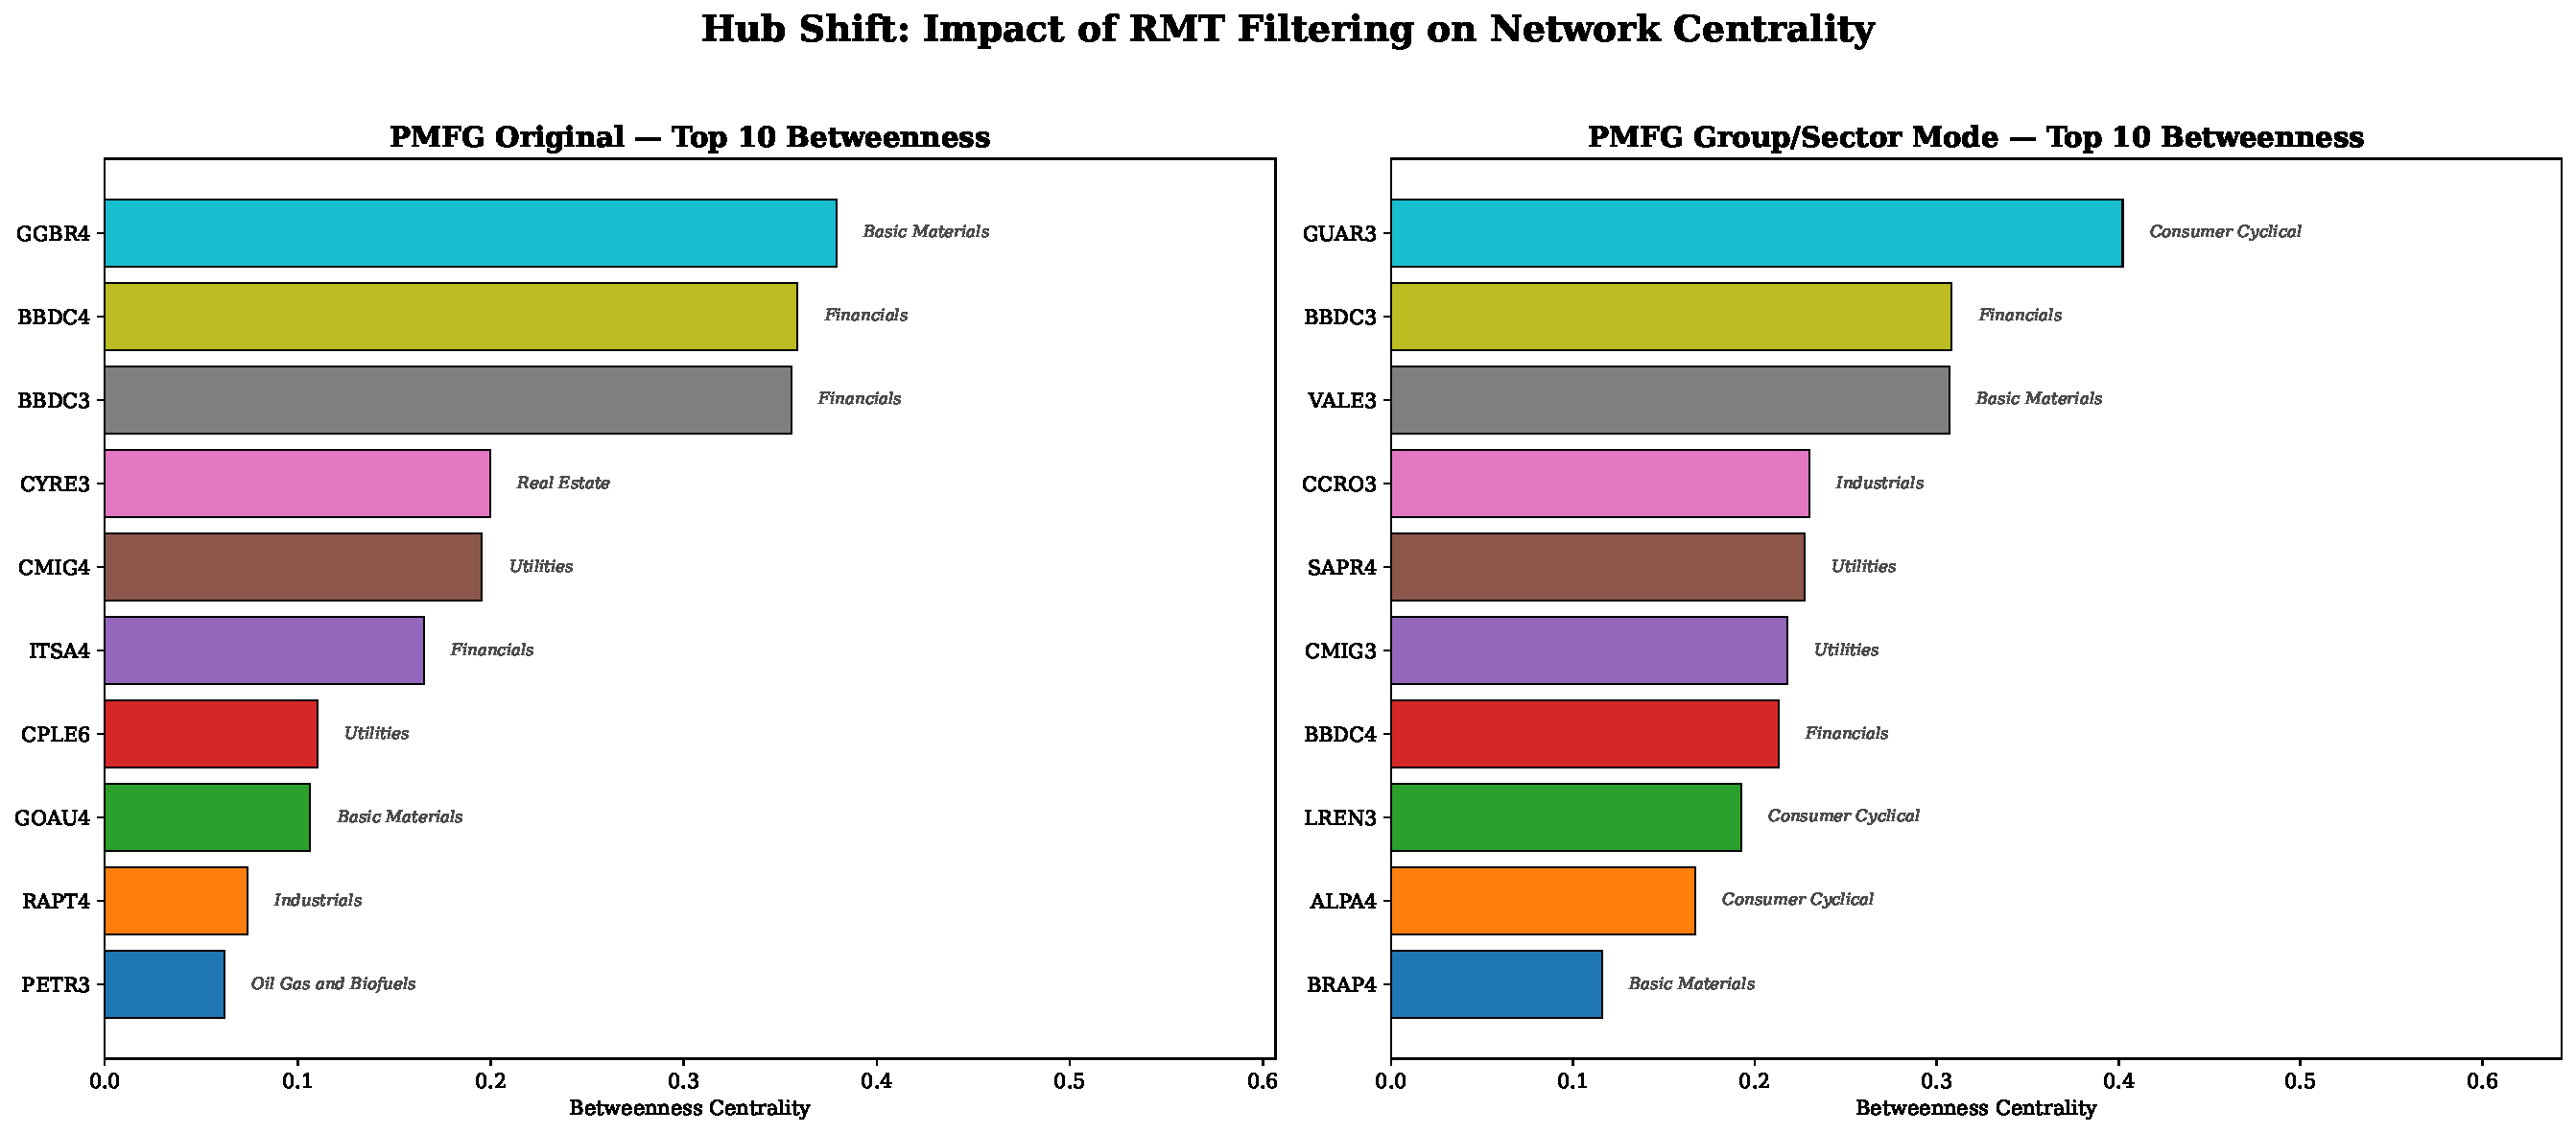
\includegraphics[
  width=\linewidth,
  height=0.58\textheight,
  keepaspectratio
]{images/figure_14_network_hub_rank_comparison.pdf}
\captionof{figure}{Hub-rank comparison across original and group-mode networks. RMT filtering changes which assets occupy central positions in the dependency topology.}
\label{fig:hub_rank}
\end{center}
